% !TEX root = MAIN.tex
\clearpage
\section{Test Suite Augmentation}
\label{sec:testGeneration}

\begin{figure}[tb]
\begin{center}
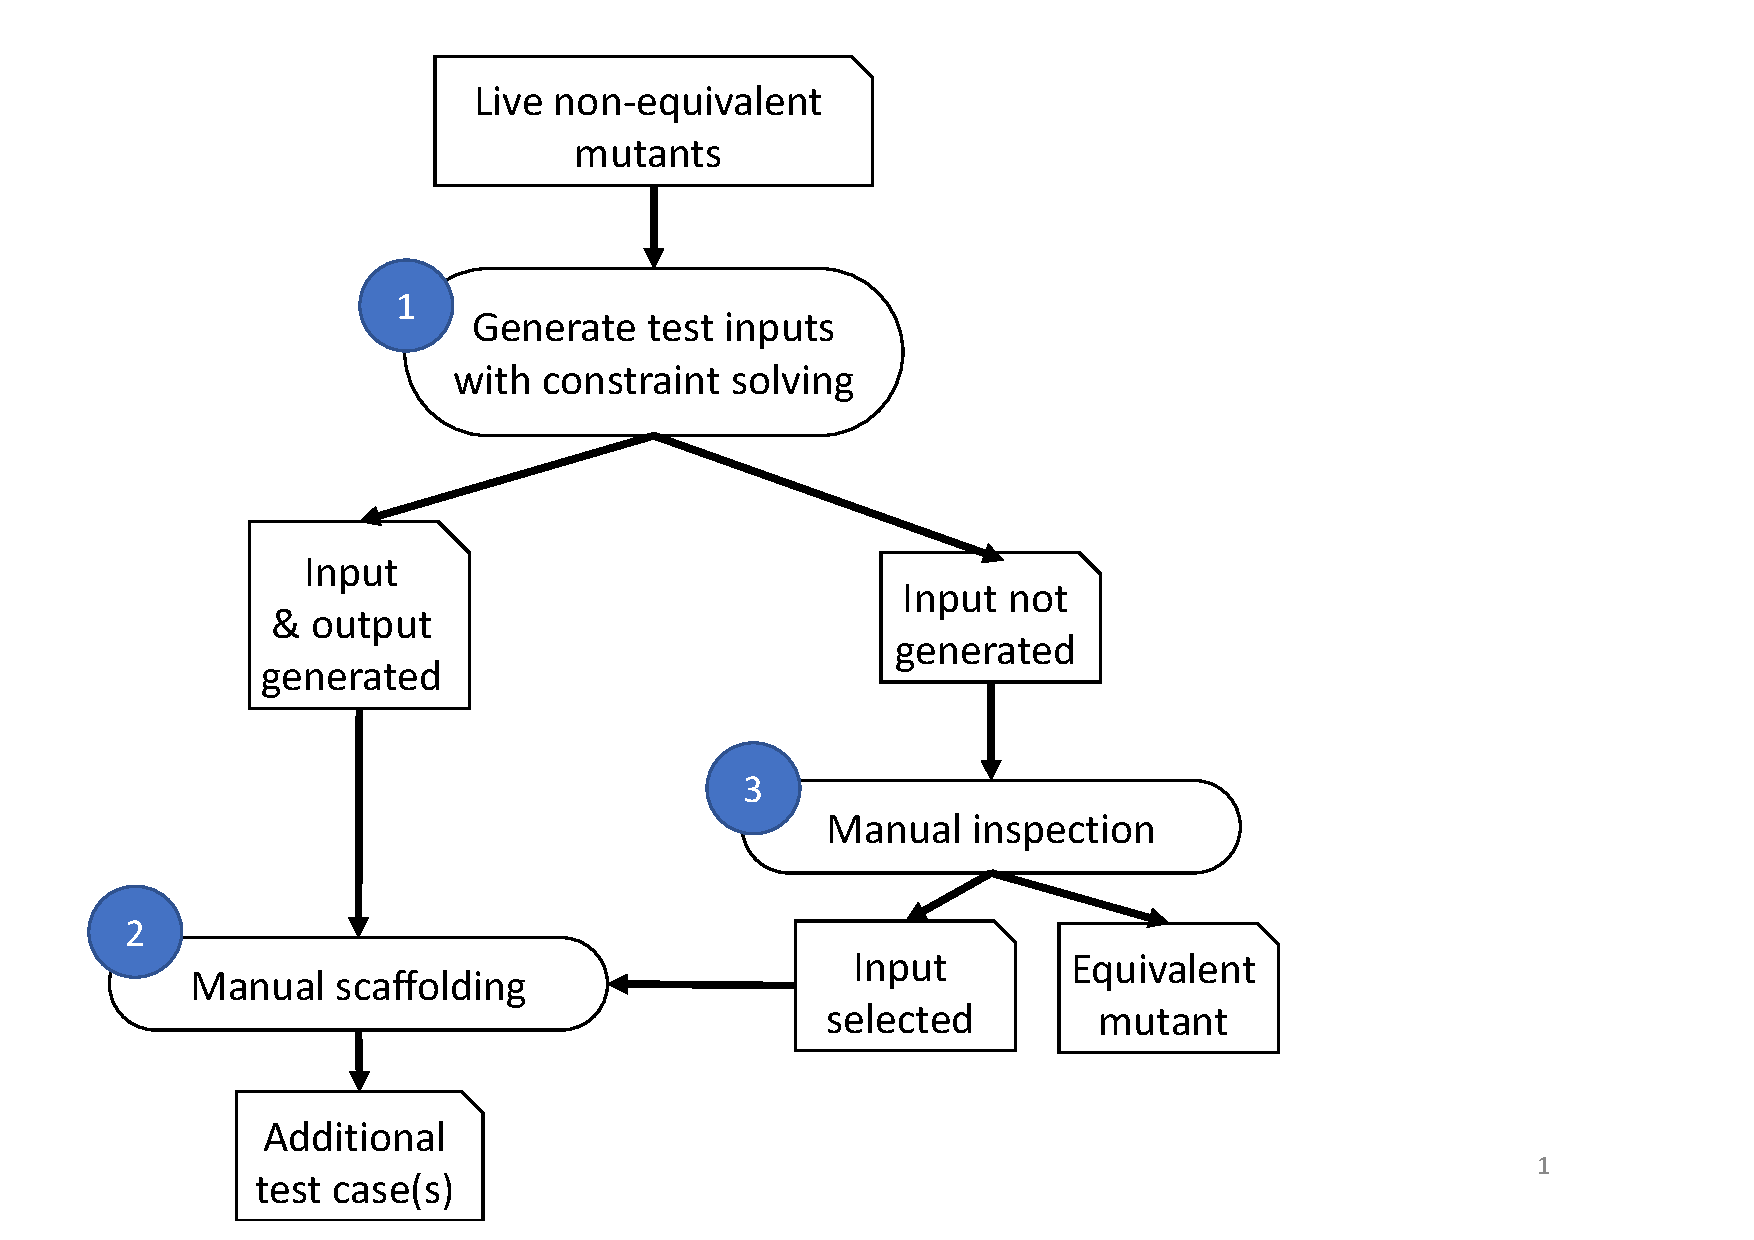
\includegraphics[width=8cm]{images/codeDrivenTestSuiteAugmentationProcess}
\caption{Overview of the proposed Test Suite Augmentation Process}
\label{fig:codeDrivenTestSuiteAugmentationProcess}
\end{center}
\end{figure}

%\TODO{This section still needs to be filled}
Figure~\ref{fig:codeDrivenTestSuiteAugmentationProcess} shows the test suite augmentation process for code-driven mutation testing.
Each live, non-equivalent mutant identified by the test suite assessment process is analyzed by means of static analysis tools based on constraint-solving (Step 1). These tools enable the identification of inputs that lead to different outputs for the original and the mutated program.
The execution of static analysis tools enable the identification of both inputs and expected outputs (i.e., the outputs that distinguish the original software from the mutant). The generated inputs and the identified outputs are used by the engineers who can manually implement a test case by reusing such inputs and outputs to define the inputs and the assertions for a test case that kills the mutant (Step 2). Mutants for which it is not possible to automatically identify a killing input needs to be manually inspcted (Step 3).


Step 1 is the only step that is automated by existing tools; anyway, it requires the definition of inputs to be processed by the specific static analysis tool to be used. In the project, two tools will be considered: CBMC and KLEE~\cite{cadar2008klee}. The process to be automated in the two cases is defined in the following subsections.

\subsection{CBMC}

% !TEX root =  ../MAIN.tex
\begin{minipage}{14cm}
\begin{lstlisting}[style=CStyle, caption=Example of code for the identification of inputs., label=GSLaugmentation]
/* Copyright (c) 2013-2017 GomSpace A/S. All rights reserved. */
  
#include <gs/util/byteorder.h>
#include <assert.h>

...

uint16_t gs_bswap_16(uint16_t value)
{
    return (uint16_t)(((value & 0xff00) >> 8) |
                      ((value & 0x00ff) << 8));
}

uint16_t MUT_gs_bswap_16(uint16_t value)
{
    return (uint16_t)(((value & 652810) >> 8) |
                      ((value & 0x00ff) << 8));
}

...

int main(){
        uint16_t v = nondet_uint16_t();
        uint16_t res;
        uint16_t resMUT;

        res = gs_bswap_16(v);
        resMUT = MUT_gs_bswap_16(v);

        __CPROVER_output("input: v", v);
        __CPROVER_output("output original: res", res);
        __CPROVER_output("output mutated: resMut", resMUT);

        assert( res == resMUT );
}
\end{lstlisting}
\end{minipage}


Listing~\ref{GSLaugmentation} shows an input file for CBMC that enables the automated identification of inputs. 
Engineers need to declare all the variables that represents inputs for the mutated function as \emph{nondet_<type>}. Function \emph{\_\_CPROVER\_output} is used to print the values identified by the execution of CBMC.

\begin{figure}[tb]
\begin{center}
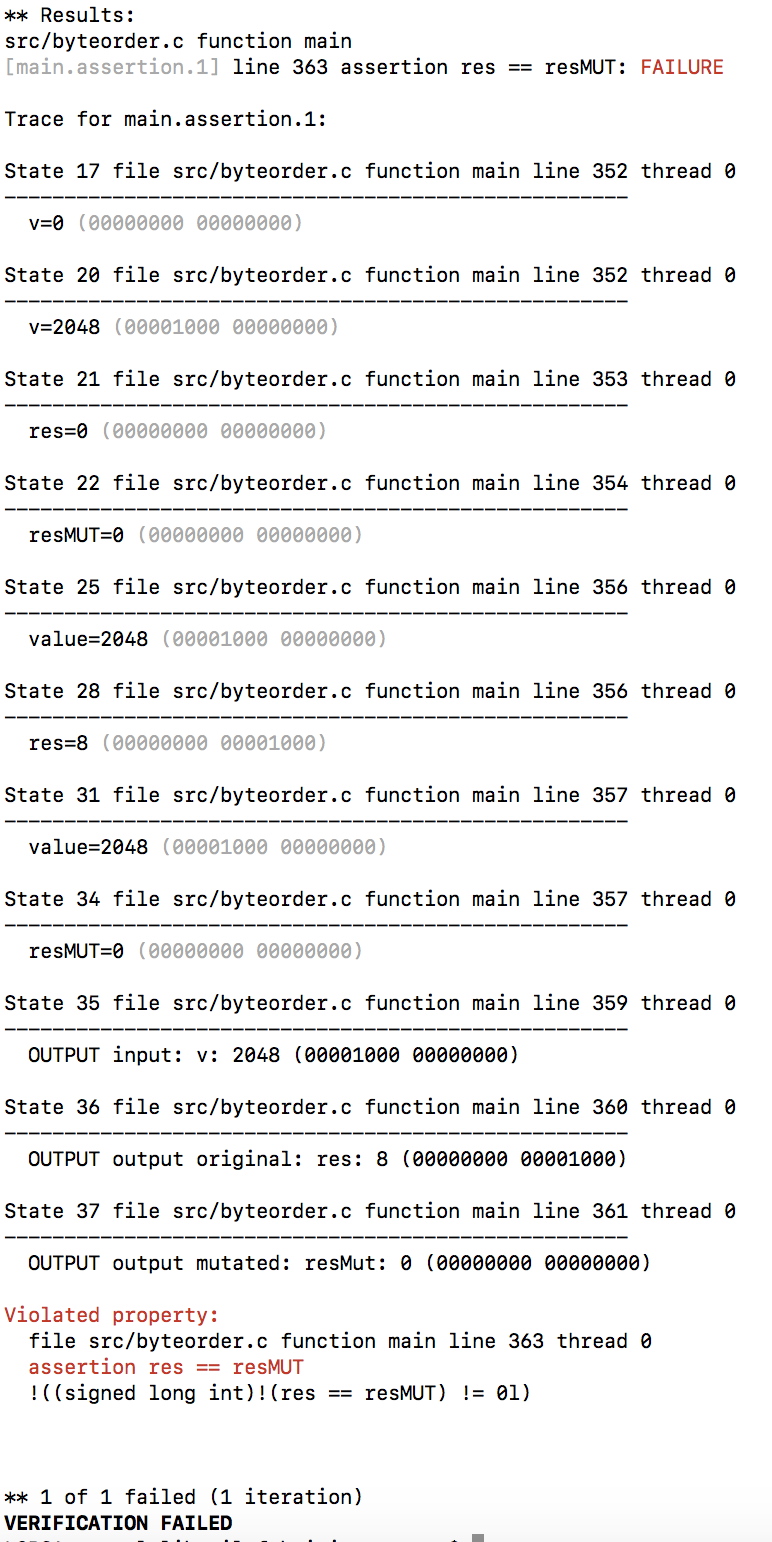
\includegraphics[width=8cm]{images/CBMCoutput}
\caption{CBMC output}
\label{fig:cbmcOutput}
\end{center}
\end{figure}